% \documentclass{article}
% \usepackage[utf8]{inputenc}

\documentclass{assignment format}
\usepackage{assignment}
\usepackage{bm}
\setcounter{section}{-1}
\setcounter{subsection}{-1}
\usepackage[cjk]{kotex}
\usepackage{amsmath, amsthm, amssymb}
\usepackage{enumerate}
\usepackage{enumitem}
\usepackage{amsfonts}
\usepackage[dvipsnames]{xcolor}
\usepackage{url}
\usepackage{graphicx}
\usepackage{float} 
\usepackage{physics}
\usepackage{bbm}
\usepackage{caption}
\usepackage{minted}
\usepackage{todonotes}
\usepackage{relsize}
\usepackage{float}
\usepackage{blindtext}
\usepackage{multicol}
\newcommand{\note}[4][]{\todo[author=#2,color=#3,size=\scriptsize,fancyline,caption={},#1]{#4}} % default note settings, used by macros below.
\newcommand{\mrinmaya}[2][]{\note[#1]{mrinmaya}{blue!40}{#2}}

\usepackage[colorlinks=true]{hyperref}

\DeclareMathOperator*{\argmax}{arg\,max}
\newcommand{\alns}[1] {
	\begin{align*} #1 \end{align*}
}

\newcommand{\pd}[2] {
 \frac{\partial #1}{\partial #2}
}
\renewcommand{\Re} { \mathbb{R} }
\newcommand{\btx} { \mathbf{\tilde{x}} }
\newcommand{\bth} { \mathbf{\tilde{h}} }
\newcommand{\smx} { \operatorname{softmax} }
\newcommand{\relu} { \operatorname{ReLU} }
\newcommand{\sigmoid} { \operatorname{\sigma} }
\newcommand{\CE} { \operatorname{CE} }
\newcommand{\byt} { \hat{\by} }
\newcommand{\yt} { \hat{y} }

\newcommand{\oft}[1]{^{(#1)}}
\newcommand{\fone}{\ensuremath{F_1}}

\newcommand{\ac}[1]{ {\color{red} \textbf{AC:} #1} }
\newcommand{\ner}[1]{\textbf{\color{blue} #1}}

\definecolor{mygreen}{rgb}{0,0.6,0}
\newcommand{\ml}[1]{\textcolor{mygreen}{\textbf{Mina:} #1}}
% real numbers R symbol
\newcommand{\Real}{\mathbb{R}}

% encoder hidden
\newcommand{\henc}{\mathbf{h}^{\text{enc}}}
\newcommand{\hencfw}[1]{\overrightarrow{\mathbf{h}^{enc}_{#1}}}
\newcommand{\hencbw}[1]{\overleftarrow{\mathbf{h}^{enc}_{#1}}}

% encoder cell
\newcommand{\cenc}{\mathbf{c}^{\text{enc}}}
\newcommand{\cencfw}[1]{\overrightarrow{\mathbf{c}^{enc}_{#1}}}
\newcommand{\cencbw}[1]{\overleftarrow{\mathbf{c}^{enc}_{#1}}}

% decoder hidden
\newcommand{\hdec}{\mathbf{h}^{\text{dec}}}

% decoder cell
\newcommand{\cdec}{\mathbf{c}^{\text{dec}}}
\newenvironment{answer}{
    {\bf Answer:} \begingroup\color{red}
}{\endgroup}%
\begin{document}


\makeheader{\textbf{Due on} Tuesday Oct. 18, 2022 \\ by \textbf{3:30pm (before class)}}{Assignment 2: Recurrent Neural Networks \& Transformers}
\begin{center}
%%%%%YOUR NAME HERE%%%%%

\fbox{%
  \parbox{\textwidth}{
  \begin{center}
\large\textbf{Honor Pledge for Graded Assignments}
\\ 
\\ 
   \large{ “I, YOUR NAME HERE , affirm that I have not given or received any unauthorized help on this assignment, and that this work is my own.”}
    \end{center}
}%
}
\end{center}

\section{Instructions (3)}
\begin{itemize}
\item Total score cannot exceed 100 points. For example, if you score 95 points from non-bonus questions and 10 points are added from bonus questions, your score will be 100 points, not 105 points.
\item You can download the skeleton code file and TeX file \href{https://github.com/yc-song/gsds-nlp-assignment-2/main}{HERE} 
\item Skeleton codes for problem 2 and 3 are at the directory \texttt{/q2} and \texttt{/q3} each. Problem 1 does not have coding problems. 
\item Run the \texttt{bash collect\_submission.sh} script to produce your 2000\_00000\_coding.zip file. Please make sure to modify collect\_sumbssion.sh file before running this command. (\textbf{2000\_00000} stands for your student id)
\item Modify this tex file into \texttt{2000\_00000\_written.pdf} with your written solutions
\item Upload both \texttt{2000\_00000\_coding.zip} and \texttt{2000\_00000\_written.pdf} to etl website. \textbf{(4pts)}
\end{itemize}

%%%NOTE FOR MYSELF%%%


% 40000 ITERATION -> 20000
% list up python files to submit
% dataset 변경
\section{NLP tasks with RNN (9+3)}
RNNs are versatile! In class, we learned that this family of neural networks have many important advantages and can be used in a variety of tasks. They are commonly used in many state-of-the-art architectures for NLP.

For each of the following tasks, state how you would run RNN to do that task. In particular, specify how the RNN would be used at test time (not training time), and specify
\begin{itemize}
    \item How many outputs i.e. number of times the softmax $\hat{y}^{(t)}$ is called from your RNN. If the number of outputs is not fixed, state it as arbitrary.  
    \item What each $\hat{y}^{(t)}$ is a probability distribution over (e.g. distributed over all species of categories)
    \item Which inputs are fed at each time step to produce each output
    \item \textbf{(Bonus) }What is one advantage that an RNN would have over a neural window-based model for this task?
    \end{itemize}
The inputs for each of the tasks are specified below.
\begin{enumerate}[label=(\alph*)]
    \item \textbf{Movie Rating (4pts)}: Classify sentiment of a movie review ranging from negative to positive (integer values from 1 to 5).\\Inputs: A sentence
    containing n words.
    \begin{answer}
    \end{answer}
    \item \textbf{Part-of-speech Tagging (4pts)}: For each word in a sentence, categorize that word in correspondence with a particular part-of-speech such as either nouns, verbs, adjectives, adverbs, etc.\\Inputs: A sentence containing n words.
    \begin{answer}
    \end{answer}
    \item \textbf{Text Generation (4pts)}: Generate text from a chatbot that was trained to speak like a news anchor by predicting the next word in the sequence. \\Input: A single start word or token that is fed into the first time step of the RNN.
    \begin{answer}
    \end{answer}
    \end{enumerate}
    

    
    

\section{GRU \& LSTM (52+6)}
\subsection{Backprop on LSTM}
In class, we learned about Long Short-Term Memory (LSTM) model. Recall the units of an LSTM cell are defined as
\begin{align*}
i_{t}=\sigma(W^{(i)}x_{t} + U^{(i)}h_{t-1})\\
f_{t}=\sigma(W^{(f)}x_{t} + U^{(f)}h_{t-1})\\
o_{t}=\sigma(W^{(o)}x_{t} + U^{(o)}h_{t-1})\\
\tilde{c_{t}} = tanh(W^{(c)}x_{t} + U^{(c)}h_{t-1})\\
c_{t} = f_{t}\circ c_{t-1}+i_{t}\circ \tilde{c_{t}}\\
h_{t}=o_{t}\circ tanh(c_{t})
\end{align*}
where the final output of the last lstm cell is defined by $\hat{y_{t}}=softmax(h_{t}W+b)$. The final cost function $J$ uses the cross-entropy loss. Consider an LSTM for two time steps, $t$ and $t-1$.
    \begin{center}
        \captionsetup{width=0.4\textwidth}
        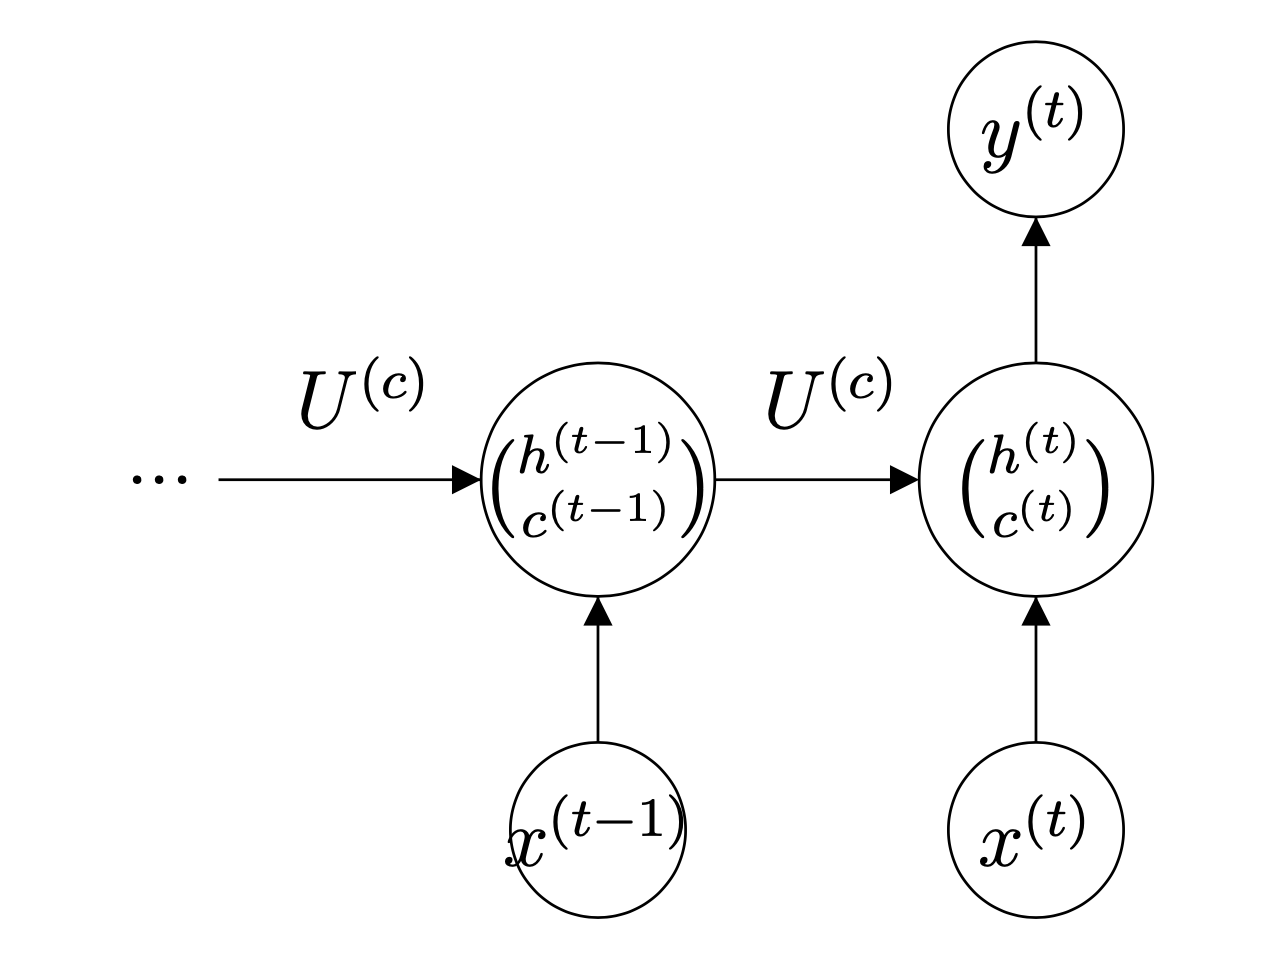
\includegraphics[width=0.4\textwidth]{LSTM.png}
        \label{LSTM-figure}
    \end{center}
\begin{enumerate}[label=(\alph*)]
    \item Derive the gradient $\frac{\delta J}{\delta U^{(c)}}$ in terms of the following gradients: $\frac{\delta h_{t}}{\delta h_{t-1}}, \frac{\delta h_{t-1}}{\delta U^{(c)}}, \frac{\delta J}{\delta h_{t}}, \frac{\delta c_{t}}{\delta U^{(c)}}, \frac{\delta c_{t-1}}{\delta U^{(c)}}, \frac{\delta c_{t}}{\delta c_{t-1}}, \frac{\delta h_{t}}{\delta c_{t}},$ and $\frac{\delta h_{t}}{\delta o_{t}}$. \textit{Not all of the gradients may be used.} You can leave the answer in the form of chain rule and do not have to calculate any individual gradients in your final result. \textbf{(3 pts)}
    \begin{answer}
    \end{answer}
    \item Which part of the gradient $\frac{\delta J}{\delta U^{(c)}}$ allows LSTM to mitigate the effect of the vanishing gradient problem? \textbf{(3 pts)}
    \begin{answer}
    \end{answer}
    \item Rather than using the last hidden state to output the sentiment of a sentence, what could be a better solution to improve the performance of the sentiment analysis task? \textbf{(3 pts)}
    \begin{answer}
    \end{answer}
\end{enumerate}
\subsection{Neural Machine Translation with LSTM}

 In Nerual Machine Translation (NMT), our goal is to convert a sentence from the \textit{source} language to the \textit{target} language. In this assignment, we will implement a sequence-to-sequence (Seq2Seq) network with attention, to build a Neural Machine Translation (NMT) system between Jeju dialect and Korean. In this section, we describe the \textbf{training procedure} for the proposed NMT system, which uses a Bidirectional LSTM Encoder and a Unidirectional LSTM Decoder. After training, you can find out how the NMT system is better than you in translating Jeju dialect. The model is trained and evaluated on JIT (Jejueo interview transcripts) dataset \footnote{https://www.kaggle.com/datasets/bryanpark/jit-dataset}
 \subsubsection{Training Procedure}
\begin{figure}[h]
    \begin{center}
        \captionsetup{width=0.8\textwidth}
        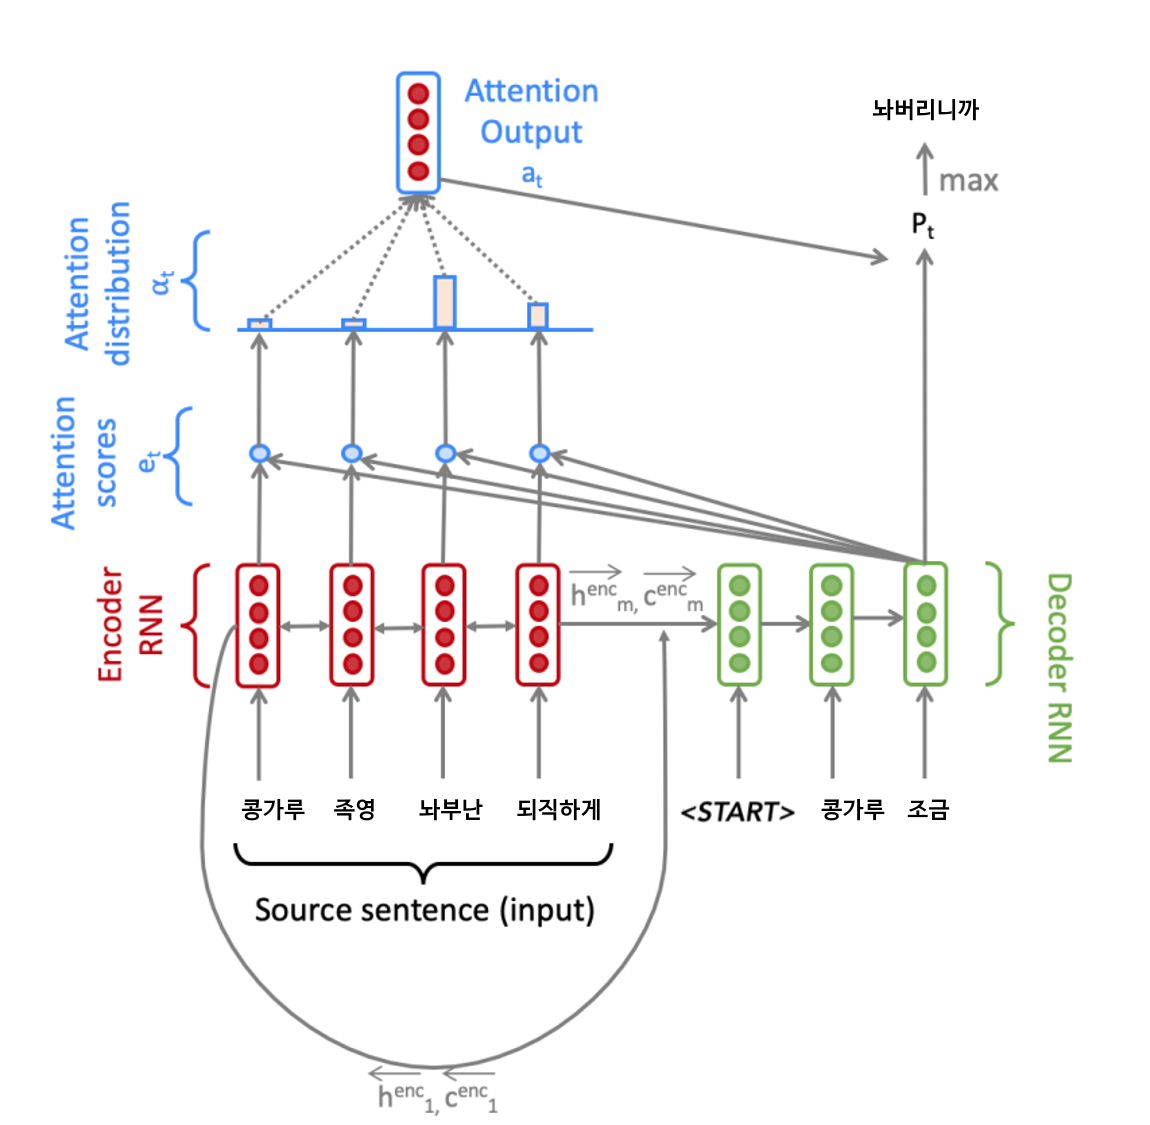
\includegraphics[width=0.7\textwidth]{nmt.png}
        \caption{Seq2Seq Model with Multiplicative Attention, shown on the third step of the decoder.  (NOTE: Embedding of NMT in the assignment differs from described above.)
        }
        \label{nmt-figure}
    \end{center}
\end{figure}
Given a sentence in the source language (Jeju dialect), we look up the subword embeddings from an embeddings matrix, yielding $\mathbf{x}_1, \dots, \mathbf{x}_m$ ($\mathbf{x}_i \in \mathbb{R}^{e \times 1}$), where $m$ is the length of the source sentence and $e$ is the embedding size. We feed these embeddings to the bidirectional encoder, yielding hidden states and cell states for both the forwards ($\rightarrow$) and backwards ($\leftarrow$) LSTMs. The forwards and backwards versions are concatenated to give hidden states $\mathbf{h}^{enc}_i$ and cell states $\mathbf{c}^{enc}_i$:

\begin{align}
    \henc_i = [\hencbw{i}; \hencfw{i}] \enspace &\text{where}\enspace \henc_i \in \Real^{2h \times 1}, \hencbw{i}, \hencfw{i} \in \Real^{h \times 1} &1 \le i \le m \\
    \cenc_i = [\cencbw{i}; \cencfw{i}] \enspace &\text{where} \enspace \cenc_i \in \Real^{2h \times 1}, \cencbw{i}, \cencfw{i} \in \Real^{h \times 1} &1 \le i \le m
\end{align}
We then initialize the decoder's first hidden state $\hdec_0$ and cell state $\cdec_0$ with a linear projection of the encoder's final hidden state and final cell state.\footnote{If it's not obvious, think about why we regard $[\hencbw{1}, \hencfw{m}]$ as the `final hidden state' of the Encoder.} 

\begin{align}
    \hdec_0 = \mathbf{W}_{h}[\hencbw{1}; \hencfw{m}] \enspace &\text{where} \enspace \hdec_0 \in \Real^{h \times 1}, \mathbf{W}_{h} \in \Real^{h \times 2h}\\
    \cdec_0 = \mathbf{W}_{c}[\cencbw{1}; \cencfw{m}] \enspace &\text{where} \enspace \cdec_0 \in \Real^{h \times 1}, \mathbf{W}_{c} \in \Real^{h \times 2h}
\end{align}


With the decoder initialized, we must now feed it a target sentence. On the $t^{th}$ step, we look up the embedding for the $t^{th}$ subword,  $\mathbf{y}_t \in \Real^{e \times 1}$. We then concatenate $\mathbf{y}_t$ with the \textit{combined-output vector} $\mathbf{o}_{t-1} \in \Real^{h \times 1}$ from the previous timestep (we will explain what this is later down this page!\@) to produce $\overline{\mathbf{y}_t} \in \Real^{(e+h) \times 1}$. Note that for the first target subword (i.e. the start token) $\mathbf{o}_{0}$ is a zero-vector. We then feed $\overline{\mathbf{y}_t}$ as input to the decoder. 

\begin{align}
    \hdec_t, \cdec_t = \text{Decoder}(\overline{\mathbf{y}_t}, \hdec_{t-1}, \cdec_{t-1}) \enspace &\text{where} \enspace \hdec_t \in \Real^{h \times 1}, \cdec_t \in \Real^{h \times 1}\\
\end{align}
We then use $\hdec_t$ to compute  multiplicative attention over $\henc_1, \dots, \henc_m$:

\begin{align}
    \mathbf{e}_{t, i} = (\hdec_t)^T\mathbf{W}_{\text{attProj}}\henc_i \enspace &\text{where} \enspace \mathbf{e}_{t} \in \Real^{m \times 1}, \mathbf{W}_{\text{attProj}}\in \Real^{h \times 2h} & 1 \le i \le m \\
    \alpha_t= \text{softmax}(\mathbf{e}_t) \enspace &\text{where} \enspace \alpha_t \in \Real^{m \times 1}\\
    \mathbf{a}_t = \sum_{i=1}^{m}\alpha_{t,i}\henc_i \enspace &\text{where} \enspace \mathbf{a}_t \in \Real^{2h \times 1}
\end{align}
 
$\mathbf{e}_{t, i}$ is a scalar, the $i$th element of $\mathbf{e}_{t} \in \Real^{m \times 1}$, computed using the hidden state of the decoder at the $t$th step, $\hdec_t \in \Real^{h \times 1}$, the attention projection $\mathbf{W}_{\text{attProj}} \in \Real^{h \times 2h}$, and the hidden state of the encoder at the $i$th step, $\henc_i \in \Real^{2h \times 1}$.

We now concatenate the attention output $\mathbf{a}_t$ with the decoder hidden state $\hdec_t$ and pass this through a linear layer, tanh, and dropout to attain the \textit{combined-output} vector $\mathbf{o}_{t}$.

\begin{align}   
    \mathbf{u}_{t} = [\mathbf{a}_{t}; \hdec_t] \enspace &\text{where} \enspace \mathbf{u}_t \in  \Real^{3h \times 1} \\
    \mathbf{v}_t = \mathbf{W}_{u}\mathbf{u}_t \enspace &\text{where} \enspace \mathbf{v}_t \in \Real^{h \times 1}, \mathbf{W}_{u} \in \Real^{h \times 3h}\\
    \mathbf{o}_t = \text{dropout}(\text{tanh}(\mathbf{v}_t)) \enspace &\text{where} \enspace \mathbf{o}_t \in \Real^{h \times 1}
\end{align}

Then, we produce a probability distribution $\mathbf{P}_t$ over target subwords at the $t^{th}$ timestep:

\begin{align}
    \mathbf{P}_t = \text{softmax}(\mathbf{W}_{\text{vocab}}\mathbf{o}_{t}) \enspace &\text{where} \enspace \mathbf{P}_t \in \Real^{V_{t} \times 1}, \mathbf{W}_{\text{vocab}} \in \Real^{V_{t} \times h}
\end{align}

Here, $V_{t}$ is the size of the target vocabulary. Finally, to train the network we then compute the cross entropy loss between $\mathbf{P}_t$ and $\mathbf{g}_{t}$, where $\mathbf{g}_{t}$ is the one-hot vector of the target subword at timestep $t$:

\begin{align}
    J_t(\theta) = \mathrm{CrossEntropy}(\mathbf{P}_t,\mathbf{g}_{t})
\end{align}

Here, $\theta$ represents all the parameters of the model and $J_t(\theta)$ is the loss on step $t$ of the decoder.
Now that we have described the model, let's try implementing it for Jeju dialect to Korean translation!

\subsubsection{Setting up Virtual Environment}
In this part, we will set up a virtual environment for implementing the NMT machine. Before you begin, make sure to read instructions about using GSDS cluster on the ETL board. Run the following commands within the assignment directory (\texttt{a2}) to create the appropriate conda environment. This guarantees that you have all the necessary packages to complete the assignment. You will be asked to implement LSTM cells and the seq2seq model using the PyTorch package. 
\begin{minted}{bash}
    bash env.sh
    conda activate a2
\end{minted}


\subsubsection{Implementation Questions}

\begin{enumerate}[label=(\alph*)]

    \item To ensure the sentences in a given batch are of the same length, we must pad shorter sentences to be the same length after identifying the longest sentence in a batch. Implement the \texttt{pad\_sents} function in \texttt{utils.py}, which returns padded sentences. \textbf{(3 pts)}
    \item Implement the code of class \texttt{LSTMCell} in the file \texttt{assignment\_code.py}. LSTMCell contains two functions: initialization \texttt{\_\_init\_\_()} and forward \texttt{forward()}. You can refer to the PyTorch documentation\footnote{LSTMCell: \url{https://pytorch.org/docs/stable/generated/torch.nn.LSTMCell.html}. GRUCell:\url{https://pytorch.org/docs/stable/generated/torch.nn.GRUCell.html}} or GRUcell class which is implemented on the skeleton code.  \textbf{(3 pts)}
   \item Implement the \texttt{\_\_init\_\_} function in \texttt{model\_embeddings.py} and \texttt{nmt\_model.py} to initialize the necessary model embeddings and layers for the NMT system. You can run sanity check by executing \texttt{python sanity\_check.py 1c} \textbf{(3 pts)}
   
    \item Implement the \texttt{encode} function in \texttt{nmt\_model.py}. This function converts the padded source sentences into the tensor $\mathbf{X}$, generates $\mathbf{h}^{enc}_1$,,,$\mathbf{h}^{enc}_m$, and computes the initial state $\mathbf{h}^{dec}_0$ and initial cell $\mathbf{c}^{dec}_0$ for the Decoder. You can run sanity check by executing \texttt{python sanity\_check.py 1d} \textbf{(3 pts)}
    \item Implement the \texttt{decode} function in \texttt{nmt\_model.py}. This function constructs $\overline{\mathbf{y}}$ 
    and runs the step function over every timestep for the input. You can run sanity check by executing \texttt{python sanity\_check.py 1e} \textbf{(3 pts)}
    \item Implement the \texttt{step} function in \texttt{nmt\_model.py}. This function applies the Decoder's LSTM cell for a single timestep, computing the encoding of the target subword $\hdec_t$, the attention scores $\mathbf{e}_t$, attention distribution $\alpha_t$, the attention output $\mathbf{a}_{t}$, and finally the combined output $\mathbf{o}_t$. You can run a non-comprehensive sanity check by executing \texttt{python sanity\_check.py 1f}  \textbf{(3 pts)}
\item Let's train the model! execute the following command:
\begin{minted}{bash}
    sh run.sh vocab
    sh run.sh train
\end{minted}
Check out the model is running on GPU when training. Training takes within one GPU hour. \textbf{(0 pts)}
    \item After training your model, execute the following command to test the model:
\begin{minted}{bash}
    sh run.sh test
\end{minted}
    To get a full credit, BLEU score should be larger than 50. \textbf{(3 pts)}
    
\end{enumerate}

\subsubsection{Written Questions}
\begin{enumerate}[label=(\alph*)]
\item The alphabet 、(\textit{araea} (아래아)), which are not used in contemporary Korean, is frequently used in jeju dialect. Because of this, conventional preprocessing tools for Korean may cause problems. Analyze \texttt{vocab.py} and state how the skeleton code fixed up the issue. \textbf{(3 pts)}
%%%Write answer here
\begin{answer}
\end{answer}

\item  \textbf{(Bonus)} As you can see in \texttt{vocab.py}, we modeled our NMT problem at a subword-level. That is, given a sentence in the source language, we looked up subword components from an embeddings matrix. Alternatively, we could have modeled the NMT problem at the word-level, by looking up whole words from the embeddings matrix. Why might it be important to model our Jejueo-to-Korean NMT problem at the subword-level vs. the whole word-level?  \textbf{(3 pts)}
\begin{answer}
\end{answer}

\item  Here we present a series of error we found in the outputs of NMT model. For each example of a reference Korean translation and NMT Korean translation, (1) please identify the error in NMT translation, (2) provide possible reasons why the model may have made the errors, and (3) Describe \textbf{ONE} possible way to fix the observed error. ($<unk>$ refers to \textit{unknown} token) \textbf{6 pts)}

\begin{enumerate}[label=(\roman*)]
\item\textbf{Source Sentence: } 가운데 대가 잇주 , 가운데 . 가운데 대 놔 가지고서 이제 만들면은 그 실 고망 , 고망 안터렐이 그 불로 무시거 불깍살로 영 헤근에 불부트민 불깍살 꺼 버리면 그디 불 잇잖느냐이 ?
 \newline
 \newline 
\textbf{Reference Translation: } 가운데 대가 있지 , 가운데 . 가운데 대 놔 가지고서 이제 만들면 그 실 구멍 , 구멍 안으로 그 불로 무엇 성냥개비로 이렇게 해서 불붙으면 성냥개비 꺼 버리면 거기 불 있잖니 ?
 \newline
 \newline
\textbf{NMT Translation: }  가운데 대가 있지 , 가운데 . 가운데 대 놔 가지고서 이제 만들면 그 실 구멍 , 구멍 안터$<unk>$이 그 불로 무엇 불깍살로 이렇게 해서 불붙으면 불깍살 거 버리면 거기 불 있잖아 ?
 \newline
\begin{answer}
\end{answer}
\item\textbf{Source Sentence: } ㅎ、ㄴ 치가 얼만곤 허민 성냥쌀 ㅎ、나가 ㅎ、ㄴ 치라 .
 \newline
 \newline 
\textbf{Reference Translation: } 한 치가 얼마인가 하면 성냥개비 하나가 한 치야 .
 \newline
 \newline
\textbf{NMT Translation: }  한 치가 얼만곤 하면 성냥개 하나가 한 치라 .
 \newline
\begin{answer}
\end{answer}
\item\textbf{Source Sentence: } 여름은 나민 저 거시기 요센 말로 난닝구 닮게시리 .
 \newline
 \newline 
\textbf{Reference Translation: }  여름은 되면 저 거시기 요샌 말로 러닝 같게끔 .
 \newline
 \newline
\textbf{NMT Translation: }   여름은 나면 저 거시기 요샌 말로 $<unk>$게끔 .
 \newline
\begin{answer}
\end{answer}
\end{enumerate}
\item You can use dot product attention, multiplicative attention, and additive attention to calculate attention score. \textbf{(4 pts)}
\begin{enumerate}[label=(\roman*)]
    \item explain ONE advantage and disadvantage of dot product attention ($\mathbf{s}^T \mathbf{h}_i$) compared to multiplicative attention ($\mathbf{s}^T\mathbf{W}\mathbf{h}_i$).
    \begin{answer}
    \end{answer}
    \item explain ONE advantage and disadvantage of dot product attention ($\mathbf{s}^T \mathbf{h}_i$) compared to additive attention ($\mathbf{v}^T \tanh(\mathbf{W_1} \mathbf{h_i}+\mathbf{W_2} \mathbf{s_t})$).
    \begin{answer}
    \end{answer}
\end{enumerate}
\item BLEU score is the most commonly used automatic evaluation metric for NMT systems. It is usually calculated across the entire test set, but here we will consider BLEU defined for a single example.\footnote{This definition of sentence-level BLEU score matches the \texttt{sentence\_bleu()} function in the \texttt{nltk} Python package. Note that the NLTK function is sensitive to capitalization. In this question, all text is lowercased, so capitalization is irrelevant. \\ \url{http://www.nltk.org/api/nltk.translate.html\#nltk.translate.bleu_score.sentence_bleu}
    }
    Suppose we have a source sentence $\mathbf{s}$, a set of $k$ reference translations $\mathbf{r}_1,\dots,\mathbf{r}_k$, and a candidate translation $\mathbf{c}$. To compute the BLEU score of $\mathbf{c}$, we first compute the \textit{modified $n$-gram precision} $p_n$ of $\mathbf{c}$, for each of $n=1,2,3,4$, where $n$ is the $n$ in \href{https://en.wikipedia.org/wiki/N-gram}{n-gram}:
    \begin{align}
        p_n = \frac{ \displaystyle \sum_{\text{ngram} \in \mathbf{c}} \min \bigg( \max_{i=1,\dots,k} \text{Count}_{\mathbf{r}_i}(\text{ngram}), \enspace \text{Count}_{\mathbf{c}}(\text{ngram}) \bigg) }{\displaystyle \sum_{\text{ngram}\in \mathbf{c}} \text{Count}_{\mathbf{c}}(\text{ngram})}
    \end{align}
     Here, for each of the $n$-grams that appear in the candidate translation $\mathbf{c}$, we count the maximum number of times it appears in any one reference translation, capped by the number of times it appears in $\mathbf{c}$ (this is the numerator). We divide this by the number of $n$-grams in $\mathbf{c}$ (denominator). \newline 

    Next, we compute the \textit{brevity penalty} BP. Let $len(c)$ be the length of $\mathbf{c}$ and let $len(r)$ be the length of the reference translation that is closest to $len(c)$ (in the case of two equally-close reference translation lengths, choose $len(r)$ as the shorter one). 
    \begin{align}
        BP = 
        \begin{cases}
            1 & \text{if } len(c) \ge len(r) \\
            \exp \big( 1 - \frac{len(r)}{len(c)} \big) & \text{otherwise}
        \end{cases}
    \end{align}
    Lastly, the BLEU score for candidate $\mathbf{c}$ with respect to $\mathbf{r}_1,\dots,\mathbf{r}_k$ is:
    \begin{align}
        BLEU = BP \times \exp \Big( \sum_{n=1}^4 \lambda_n \log p_n \Big)
    \end{align}
    where $\lambda_1,\lambda_2,\lambda_3,\lambda_4$ are weights that sum to 1. The $\log$ here is natural log.
    \newline
    \begin{enumerate}[label=(\roman*)]
        \item Consider this example.
        \begin{itemize}
\item        Source Sentence $\mathbf{s}$: \textbf{그때는 뭐 사먹을 것도 엇일 때고 주로 뭐 학습장이나 작기장이나 사던지 그렇게 헤엇던 거 가따} 
      \item  Reference Translation $\mathbf{r}_1$: 그때는 뭐 사먹을 것도 없을 때고 주로 뭐 학습장이나 종합장이나 사던지 그렇게 했었던 거 같아 
        \item Reference Translation $\mathbf{r}_2$: 그때는 뭐 사먹을 것도 없을 시절이고 주로 뭐 학습장이나 잡기장이나 사든지 그렇게 했었던 거 같다 
        \item NMT Translation $\mathbf{c}_1$: 그때는 뭐 사먹을 것도 없을 때고 주로 뭐 학습장이나 작기장이나 사든지 그렇게 했었던 거 가
    \end{itemize}

    Please compute the BLEU scores for $\mathbf{c}_1$. Let $\lambda_i=0.5$ for $i\in\{1,2\}$ and $\lambda_i=0$ for $i\in\{3,4\}$ (\textbf{this means we ignore 3-grams and 4-grams}, i.e., don't compute $p_3$ or $p_4$). When computing BLEU scores, show your working (i.e., show your computed values for $p_1$, $p_2$, $len(c)$, $len(r)$ and $BP$). Note that the BLEU scores can be expressed between 0 and 1 or between 0 and 100. The code is using the 0 to 100 scale while in this question we are using the \textbf{0 to 1} scale. \textbf{(6 pts)}
    \begin{answer}
    \end{answer}
    \item Due to data availability, NMT systems are often evaluated with respect to only a single reference translation. Please explain (in a few sentences) why this may be problematic. In your explanation, discuss how the BLEU score metric assesses the quality of NMT translations when there are multiple reference transitions versus a single reference translation. \textbf{(3 pts)}
    \begin{answer}
    \end{answer}
    \item \textbf{(BONUS)} List ONE advantage and disadvantage of BLEU, compared to human evaluation, as an evaluation metric for Machine Translation. \textbf{(3 pts)}
    \begin{answer}
    \end{answer}
    \end{enumerate}
\end{enumerate}


\section{Transformer (36)}
\subsection{Attention Exploration}

Multi-headed self-attention is the core modeling component of Transformers.
In this question, we'll get some practice working with the self-attention equations, and motivate why multi-headed self-attention can be preferable to single-headed self-attention.

Recall that attention can be viewed as an operation on a \textit{query} $q\in\mathbb{R}^d$, a set of \textit{value} vectors $\{v_1,\dots,v_n\}, v_i\in\mathbb{R}^d$, and a set of \textit{key} vectors $\{k_1,\dots,k_n\}, k_i \in \mathbb{R}^d$, specified as follows:
\begin{align}
&c = \sum_{i=1}^{n} v_i \alpha_i \\
&\alpha_i = \frac{\exp(k_i^\top q)}{\sum_{j=1}^{n} \exp(k_j^\top q)}
\end{align} 
with $\alpha_i$ termed the ``attention weights''. 
Observe that the output $c\in\mathbb{R}^d$ is an average over the value vectors weighted with respect to $\alpha_i$.
\newline
\textbf{NOTE}: Do not take this problem so seriously. Every answer can be stated within 5 lines! 

\begin{enumerate}[label=(\alph*)]


\item\textbf{An average of two.} 
A Transformer model might want to incorporate information from \textit{multiple} source vectors. 
Consider the case where we want to incorporate information from \textbf{two} vectors $v_a$ and $v_b$, with corresponding key vectors $k_a$ and $k_b$.
\begin{enumerate}[label=(\roman*)]
\item How should we combine two $d$-dimensional vectors $v_a, v_b$ into one output vector $c$ in a way that preserves information from both vectors? 
In machine learning, one common way to do so is to take the average: $c = \frac{1}{2} (v_a + v_b)$.
It might seem hard to extract information about the original vectors $v_a$ and $v_b$ from the resulting $c$, but under certain conditions one can do so. In this problem, we'll see why this is the case.
\\ \\
Suppose that although we don't know $v_a$ or $v_b$, we do know that $v_a$ lies in a subspace $A$ formed by the $m$ basis vectors $\{a_1, a_2, \ldots, a_m\}$, while $v_b$ lies in a subspace $B$ formed by the $p$ basis vectors $\{b_1, b_2, \ldots, b_p\}.$ (This means that any $v_a$ can be expressed as a linear combination of its basis vectors, as can $v_b$. All basis vectors have norm 1 and orthogonal to each other.)
Additionally, suppose that the two subspaces are orthogonal; i.e. $a_j^\top b_k = 0$ for all $j, k$.

Using the basis vectors $\{a_1, a_2, \ldots, a_m\}$, construct a matrix $M$ such that for arbitrary vectors $v_a \in A$ and $v_b \in B$, we can use $M$ to extract $v_a$ from the sum vector $s = v_a + v_b$. In other words, we want to construct $M$ such that for any $v_a, v_b$,  $Ms = v_a$).

\textbf{Note:} both $M$ and $v_a, v_b$ should be expressed as a vector in $\mathbb{R}^d$, not in terms of vectors from $A$ and $B$. \\

\textbf{Hint:} Given that the vectors $\{a_1, a_2, \ldots, a_m\}$ are both \textit{orthogonal} and \textit{form a basis} for $v_a$, we know that there exist some $c_1, c_2, \ldots, c_m$ such that $v_a = c_1 a_1 + c_2 a_2 + \cdots + c_m a_m$. Can you create a vector of these weights $c$? \textbf{(3 pts)}

\begin{answer}
\end{answer}

\item As before, let $v_a$ and $v_b$ be two value vectors corresponding to key vectors $k_a$ and $k_b$, respectively.
Assume that (1) all key vectors are orthogonal, so $k_i^\top k_j = 0$ for all $i \neq j$; and (2) all key vectors have norm $1$.\footnote{Recall that a vector $x$ has norm 1 iff $x^\top x = 1$.}
\textbf{Find an expression} for a query vector $q$ such that $c \approx \frac{1}{2}(v_a + v_b)$. \newline \textbf{(HINT: } while the softmax function will never \textit{exactly} average the two vectors, you can get close by using a large scalar multiple in the expression.) \textbf{(3 pts)}
\begin{answer}
\end{answer}
\end{enumerate}

\item\textbf{Drawbacks of single-headed attention:} \label{q_problem_with_single_head}
In the previous part, we saw how it was \textit{possible} for a single-headed attention to focus equally on two values.
The same concept could easily be extended to any subset of values.
In this question we'll see why it's not a \textit{practical} solution.
Consider a set of key vectors $\{k_1,\dots,k_n\}$ that are now randomly sampled, $k_i\sim \mathcal{N}(\mu_i, \Sigma_i)$, where the means $\mu_i \in \mathbb{R}^d$ are known to you, but the covariances $\Sigma_i$ are unknown.
Further, assume that the means $\mu_i$ are all perpendicular; $\mu_i^\top \mu_j = 0$ if $i\not=j$, and unit norm, $\|\mu_i\|=1$.

\begin{enumerate}[label=(\roman*)]
\item Assume that the covariance matrices are $\Sigma_i = \alpha I \forall i \in \{1, 2, \ldots, n\}$, for vanishingly small $\alpha$.
Design a query $q$ in terms of the $\mu_i$ such that as before, $c\approx \frac{1}{2}(v_a + v_b)$, and provide a brief argument as to why it works. \textbf{(3 pts)}
\begin{answer}
\end{answer}

\item Though single-headed attention is resistant to small perturbations in the keys, some types of larger perturbations may pose a bigger issue. Specifically, in some cases, one key vector $k_a$ may be larger or smaller in norm than the others, while still pointing in the same direction as $\mu_a$. As an example, let us consider a covariance for item $a$ as $\Sigma_a = \alpha I + \frac{1}{2}(\mu_a\mu_a^\top)$ for vanishingly small $\alpha$ (as shown in figure \ref{ka_plausible}). This causes $k_a$ to point in roughly the same direction as $\mu_a$, but with large variances in magnitude. Further, let $\Sigma_i = \alpha I$ for all $i \neq a$.
\begin{figure}[h]
\centering
\captionsetup{justification=centering,margin=2cm}
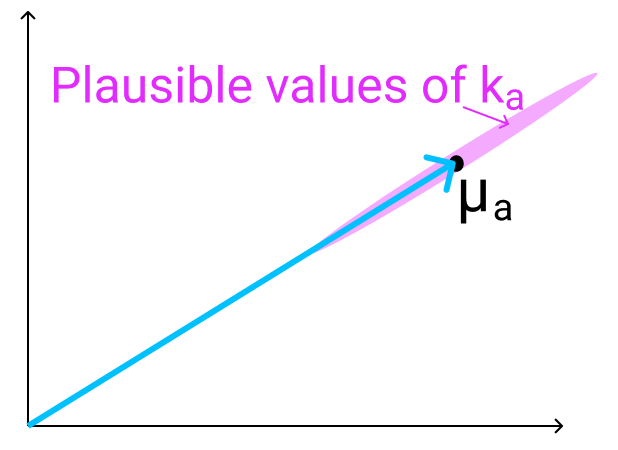
\includegraphics[width=0.35\linewidth]{ka_plausible.png}
\caption{The vector $\mu_a$ (shown here in 2D as an example), with the range of possible values of $k_a$ shown in red. As mentioned previously, $k_a$ points in roughly the same direction as $\mu_a$, but may have larger or smaller magnitude.}
\label{ka_plausible}
\end{figure}

When you sample $\{k_1,\dots,k_n\}$ multiple times, and use the $q$ vector that you defined in part i., what qualitatively do you expect the vector $c$ will look like for different samples? \textbf{(3 pts)}

\begin{answer}
\end{answer}
\end{enumerate}

\item \textbf{Benefits of multi-headed attention:}
Now we'll see some of the power of multi-headed attention.
We'll consider a simple version of multi-headed attention which is identical to single-headed self-attention as we've presented it in this homework, except two query vectors ($q_1$ and $q_2$) are defined, which leads to a pair of vectors ($c_1$ and $c_2$), each the output of single-headed attention given its respective query vector.
The final output of the multi-headed attention is their average, $\frac{1}{2}(c_1+c_2)$.
As in question 1(\ref{q_problem_with_single_head}), consider a set of key vectors $\{k_1,\dots,k_n\}$ that are randomly sampled, $k_i\sim \mathcal{N}(\mu_i, \Sigma_i)$, where the means $\mu_i$ are known to you, but the covariances $\Sigma_i$ are unknown.
Also as before, assume that the means $\mu_i$ are mutually orthogonal; $\mu_i^\top \mu_j = 0$ if $i\not=j$, and unit norm, $\|\mu_i\|=1$.
\begin{enumerate}[label=(\roman*)]
\item
Assume that the covariance matrices are $\Sigma_i=\alpha I$, for vanishingly small $\alpha$.
Design $q_1$ and $q_2$ such that $c$ is approximately equal to $\frac{1}{2}(v_a+v_b)$. \textbf{(3 pts)}

\begin{answer}
\end{answer}

\item
Assume that the covariance matrices are $\Sigma_a=\alpha I + \frac{1}{2}(\mu_a\mu_a^\top)$ for vanishingly small $\alpha$, and $\Sigma_i=\alpha I$  for all $i \neq a$.
Take the query vectors $q_1$ and $q_2$ that you designed in part i.
What, qualitatively, do you expect the output $c$ to look like across different samples of the key vectors? Please briefly explain why. You can ignore cases in which $k_a^\top q_i < 0$. \textbf{(3 pts)}

\begin{answer}
\end{answer}
\end{enumerate}
\end{enumerate}
\subsection{Implement Minimalist Version of BERT}
In this assignment, you will implement some important components of the BERT model to better understand its architecture. You will then perform sentence classification with the model you implemented. There are no written questions in this section. For more details about transformer architecture, please refer to the paper \textit{Attention is all you need}: \url{https://arxiv.org/pdf/1706.03762.pdf} \newline
Run \texttt{setup.sh} to properly set up the environment. You are NOT allowed to use external libraries such as \texttt{transformers} in torch. 

\begin{figure}[h]
\centering
\captionsetup{justification=centering,margin=2cm}
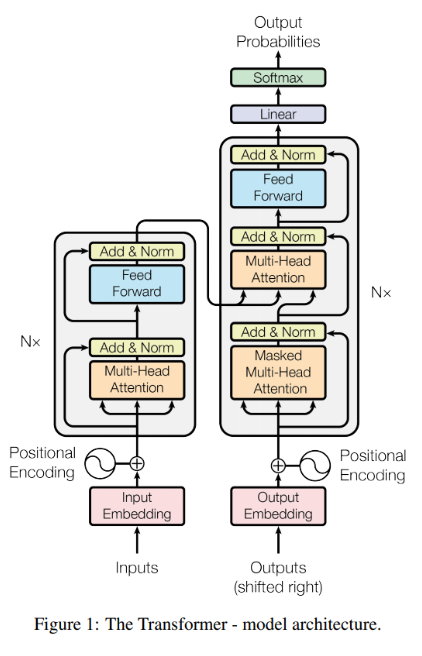
\includegraphics[width=0.35\linewidth]{transformer.png}
\caption{Model architecture of the transformer}
\label{transformer}
\end{figure}
\begin{enumerate}[label=(\alph*)]

    \item Implement \texttt{attention} function in \texttt{BertSelfAttention} class of \texttt{bert.py}. Scaled dot-product attention are computed as below: 
        \begin{align}
\text{Attention}(Q,K,V) = \text{softmax}(\frac{QK^T}{\sqrt{d_k}})V
\end{align} \textbf{(3 pts)}
    \item Implement \texttt{add\_norm} function in \texttt{BertLayer} class of \texttt{bert.py}. It corresponds to Add \& Norm Layer in the figure \ref{transformer}, which is defined as $\text{LayerNorm}(x+\text{Sublayer}(x))$ \textbf{(3 pts)}
    \item  Implement \texttt{forward} function in \texttt{BertLayer} class of \texttt{bert.py}. It corresponds to encoder stacks which are described on the left of the figure \ref{transformer}. After completing the codes, run \texttt{python sanity\_check.py} to check your implementation. \textbf{(3 pts)}
   \item  Implement \texttt{step} function in \texttt{AdamW} class of \texttt{optimizer.py}. Implement parameter update of Adam optimizer. For sanity check, run \texttt{python optimizer\_test.py} \textbf{(3 pts)}
       \newline (as noted at skeleton codes, we are using the optimizer presented at \href{https://arxiv.org/abs/1412.6980}{THIS PAPER}) 
  \item  Implement \texttt{train} function in \texttt{classifier.py}. This function carries out backpropagation through the model parameters. \textbf{(3 pts)}
  
   \item Show time! Run \texttt{python3 classifier.py --option finetune --epochs NUM\_EPOCHS --lr LR --train data/sst-train.txt --dev data/sst-dev.txt --test data/sst-test.txt --use\_gpu} . Report hyperparameters NUM\_EPOCHS and LR which shows test accuracy higher than 0.5 and submit \textbf{ONE} \texttt{.pt} file accordingly. \newline \textbf{(HINT: }Think about how learning rate is likely to be when fine-tune the transformer model) \textbf{(3 pts)} \begin{answer}
   \end{answer}
\end{enumerate}

\end{document}
